\chapter{Chaînes de Markov en temps discret}

\section{Chaînes de Markov}

\begin{definition}
    Un processus stochastique est une collection $\{X_t\mid t\in T\}$ de v.a sur un espace $(\Omega,\mathcal{A}, P)$, indexée par un ensemble $T$. Lorsque $T= \N$, on parle de processus stochastique en temps discret et lorsque $T= \R ^{\ge0}$, on parle de processus stochastique en temps continu.
\end{definition}

On veut s'éloigner de la notion i.i.d. que l'on a pu étudier auparavant dans le but d'étudier des phenomenes plus complexes.

\begin{definition}
    Une chaine de Markov (en temps discret) est un processus stochastique $\{X_n\mid n\ge 0\}$ à valeurs dasn un ensemble fini ou dénombrable $E$, qui satisfait :
    \begin{description}
        \item[Propriété de Markov : ]$$ P(X_{n+1}\mid X_0 = i_0, X_1 = i_1,\dotsc, X_n = i_n) = P(X_{n+1} = j\mid X_n = i_n) \quad \forall n \in \N, \forall j, i_0, \dotsc, i_n\in E$$ 
        \item[Homogéneité : ] $$P(X_{n+1}= j\mid X_n = 1)= P(X_1= j\mid X_0= i) \quad \forall n, \forall i,j \in E$$    
    \end{description}
\end{definition}
\begin{notation}
    $E = \{\text{états du système\}}$
    $X_n = i$ : le système est dans l'état $i$ au moment $n$.
    $X_n = i, X_{n=1} = j$ : entre $n$ et $n+1$, le système fait une transitino de $i$ à $j$
    Un vecteur sera noté $\overline{v}$ et sa nature dépendra du contexte. On utilise aussi les conventions suivantes : $\frac{1}{\infty}= 0$ et $0\cdot \infty = 0$.
\end{notation}

\begin{definition}
    La matrice de transition d'une chaîne de Markov $\{X_n\}$ est la matrice $\underline P$ de dimension $\abs{E}\times\abs{E}$ telle que $\un P_{ij} = P(X_1 = j\mid X_0 = i) = P(X_{n+1} = j\mid X_n = i)\quad \forall n$
\end{definition}

On dit aussi que $\underline P$ sera une matrice stochastique, c'est à dire que 
\begin{itemize}
    \item $P_{ij}\geq 0 \quad \forall i,j \in E$
    \item $\un P\overline{1}= \overline{ 1}$
\end{itemize}
Pour être clair :
$$(\un P\overline{1})_i= \sum_{k \in E}P_{ik}= \sum _{k\in E}P(X_1= k\mid X_0= i)= P(X_1\in E\mid X_0= i)= 1$$

\begin{definition}
    Le vecteur initial $\overline{\alpha}$ d'une CM $\{X_n\}$ est le vecteur de dim $|E|$ tel que $$\alpha_i= P(X_0= i)$$
    En fait, $\overline{\alpha}$ approxime la loi de la v.a de $X_0$ 
\end{definition}
\begin{proposition}
     Le couple $(\overline{\alpha},P)$ caractérise complètement l'évolution de la CM.
    \begin{enumerate}
        \item $$P(X_0 = i_0, X_1 = i_1,\dotsc, X_n = i_n) = \alpha_{i_0}P_{i_0i_1}P_{i_1i_2}\cdot\dots P_{i_{n-1}i_n}$$
        \item $$P(X_n= j\mid X_0= i)= (\un P^n)_{ij}$$
        \item $$P(X_n= j)= (\overline{\alpha}\un P^n)_j$$
    \end{enumerate}
\end{proposition}

Pour rappel: 
$$P(A\cap B \mid C)= P(A\mid B,C)P(B\mid C)$$

\begin{proof}
    \begin{enumerate}
        \item \begin{align*}
           P(X_0 = \dotsc, X_n = i_n) &= P( X_1 = i_1,\dotsc, X_n = i_n\mid X_0 = i_0)P(X_0 = i_0)\\
           &=  P(X_2 = i_2,\dots, X_n = i_n\mid X_0 = i_0, X_1 = i_1)P(X_1 = i_1\mid X_0 = i_0) \alpha_{i_0}\\
           &=  P(X_3 = i_3,\dots, X_n = i_n\mid X_0 = i_0, X_1 = i_1,X_2 = i_2)P(X_2 = i_2\mid X_0 = i_0, X_1 = i_1) \un P_{01}\alpha_{i_0}\\
           &= P(X_3 = i_3,\dots, X_n = i_n\mid X_0 = i_0, X_1 = i_1,X_2 = i_2)P(X_2 = i_2\mid  X_1 = i_1) \un P_{01}\alpha_{i_0} \text{ par la propriété de Markov}
           &= \dots\\ =\alpha_{i_0}P_{i_0i_1}P_{i_1i_2}\cdot\dots P_{i_{n-1}i_n}
        \end{align*}
        \item Par induction sur $n$. Le cas de base est trivialement vérifié. Supposons que cela est vrai pour $n$ montrons le pour $n+1$
        \begin{align*}
        P(X_{n+1}=j \mid X_0= i)&=\sum_{k\in E}P(X_{n+1}=j\mid X_0=i, X_n=k)P(X_n= k\mid X_0= i)\\
        & = \sum _{k\in E}(P^n)_{ik}P_{kj}\\
        &=(P^n P)_{ij}
        \\ &= (P^{n+1})_{ij}
        \end{align*}
        \item 
        \begin{align*}
            P(X_n = j)&= \sum_{k\in E}P(X_n = j\mid X_0= k)P(X_0= k)\\ &= \sum _{k\in E} (P^{n})_{kj}\alpha_k\\
            &= (\overline{\alpha}P^n)_j
        \end{align*}
    \end{enumerate}
\end{proof}
\begin{proposition}[Équations de Chapman-Kolmogorov]
    $$P(X_{n+m} = j\mid X_0 = i) = \sum {k\in E}(P(X_n = k\mid X_0 = i)P(X_m = j\mid X_0 = k)$$
\end{proposition}
\begin{proof}
    
\end{proof}
On sait que $P^{n+m}= P^nP ^m$. On sait donc toujours que 
$$P(X_{n+m}= j \mid X_0 = i)= \sum_{k\in E}P(X_n= k\mid X_0= i)P(X_m= j \mid X_0= k)$$
\begin{exemple}
Voici quelques exemples de CM : 
    \begin{itemize}
        \item Tous les jours on a un état que qui s'appel $S$ pour soleil $N$ pour nuage et $p$ pour pluie. Et le temps qu'il fait demain est uniquement dépendant du temps de ce jour. Si disons, on sait que : aujourd'hui il fait soleil alors demain ce sera pluie (80\%) et nuage (20\%) et s'il fait nuageux alors demain soleil (30\%) et nuage pour 70\% et enfin si aujourd'hui on est dans l'état pluie  alors il fait du soleil pour 5\%, nuage pour 5\% et pluie pour 90\%
        
\begin{center}


\tikzset{every picture/.style={line width=0.75pt}} %set default line width to 0.75pt        

\begin{tikzpicture}[x=0.75pt,y=0.75pt,yscale=-1,xscale=1]
%uncomment if require: \path (0,300); %set diagram left start at 0, and has height of 300

%Shape: Circle [id:dp33196130673660107] 
\draw   (180,100.33) .. controls (180,83.03) and (194.03,69) .. (211.33,69) .. controls (228.64,69) and (242.67,83.03) .. (242.67,100.33) .. controls (242.67,117.64) and (228.64,131.67) .. (211.33,131.67) .. controls (194.03,131.67) and (180,117.64) .. (180,100.33) -- cycle ;
%Shape: Circle [id:dp014015497053411319] 
\draw   (291,220.33) .. controls (291,203.03) and (305.03,189) .. (322.33,189) .. controls (339.64,189) and (353.67,203.03) .. (353.67,220.33) .. controls (353.67,237.64) and (339.64,251.67) .. (322.33,251.67) .. controls (305.03,251.67) and (291,237.64) .. (291,220.33) -- cycle ;
%Shape: Circle [id:dp6807025049126726] 
\draw   (360,105.33) .. controls (360,88.03) and (374.03,74) .. (391.33,74) .. controls (408.64,74) and (422.67,88.03) .. (422.67,105.33) .. controls (422.67,122.64) and (408.64,136.67) .. (391.33,136.67) .. controls (374.03,136.67) and (360,122.64) .. (360,105.33) -- cycle ;
%Curve Lines [id:da7122821084349672] 
\draw    (204.67,67.4) .. controls (311.05,-3.52) and (355.33,54.6) .. (389.77,73.18) ;
\draw [shift={(391.33,74)}, rotate = 206.92] [color={rgb, 255:red, 0; green, 0; blue, 0 }  ][line width=0.75]    (10.93,-3.29) .. controls (6.95,-1.4) and (3.31,-0.3) .. (0,0) .. controls (3.31,0.3) and (6.95,1.4) .. (10.93,3.29)   ;
%Curve Lines [id:da6248679396945833] 
\draw    (226.67,125.4) .. controls (270.89,152.53) and (360.19,170.7) .. (390.44,137.68) ;
\draw [shift={(391.33,136.67)}, rotate = 130.45] [color={rgb, 255:red, 0; green, 0; blue, 0 }  ][line width=0.75]    (10.93,-3.29) .. controls (6.95,-1.4) and (3.31,-0.3) .. (0,0) .. controls (3.31,0.3) and (6.95,1.4) .. (10.93,3.29)   ;
%Curve Lines [id:da9052624080954654] 
\draw    (398,74) .. controls (437.6,44.3) and (469.03,77.72) .. (424.05,104.52) ;
\draw [shift={(422.67,105.33)}, rotate = 330.19] [color={rgb, 255:red, 0; green, 0; blue, 0 }  ][line width=0.75]    (10.93,-3.29) .. controls (6.95,-1.4) and (3.31,-0.3) .. (0,0) .. controls (3.31,0.3) and (6.95,1.4) .. (10.93,3.29)   ;
%Curve Lines [id:da09663037780473371] 
\draw    (189.67,123.4) .. controls (113.29,123.46) and (264.75,238.43) .. (289.05,232.13) ;
\draw [shift={(290.67,231.4)}, rotate = 144.16] [color={rgb, 255:red, 0; green, 0; blue, 0 }  ][line width=0.75]    (10.93,-3.29) .. controls (6.95,-1.4) and (3.31,-0.3) .. (0,0) .. controls (3.31,0.3) and (6.95,1.4) .. (10.93,3.29)   ;
%Curve Lines [id:da7732277560879418] 
\draw    (293.67,200.4) .. controls (295.3,170.41) and (245.71,150.22) .. (221.14,135.31) ;
\draw [shift={(219.67,134.4)}, rotate = 32.01] [color={rgb, 255:red, 0; green, 0; blue, 0 }  ][line width=0.75]    (10.93,-3.29) .. controls (6.95,-1.4) and (3.31,-0.3) .. (0,0) .. controls (3.31,0.3) and (6.95,1.4) .. (10.93,3.29)   ;
%Curve Lines [id:da7553000998414746] 
\draw    (342,198) .. controls (431.38,185.71) and (411.75,156.89) .. (409.78,131.36) ;
\draw [shift={(409.67,129.4)}, rotate = 87.8] [color={rgb, 255:red, 0; green, 0; blue, 0 }  ][line width=0.75]    (10.93,-3.29) .. controls (6.95,-1.4) and (3.31,-0.3) .. (0,0) .. controls (3.31,0.3) and (6.95,1.4) .. (10.93,3.29)   ;
%Curve Lines [id:da7057746669417809] 
\draw    (307.67,250.4) .. controls (305.36,274.56) and (344.86,297.93) .. (340.8,247.94) ;
\draw [shift={(340.67,246.4)}, rotate = 84.51] [color={rgb, 255:red, 0; green, 0; blue, 0 }  ][line width=0.75]    (10.93,-3.29) .. controls (6.95,-1.4) and (3.31,-0.3) .. (0,0) .. controls (3.31,0.3) and (6.95,1.4) .. (10.93,3.29)   ;

% Text Node
\draw (274,6.4) node [anchor=north west][inner sep=0.75pt]    {$ \begin{array}{l}
0,2\\
\end{array}$};
% Text Node
\draw (279,128.4) node [anchor=north west][inner sep=0.75pt]    {$0,3$};
% Text Node
\draw (454,70.4) node [anchor=north west][inner sep=0.75pt]    {$ \begin{array}{l}
0,7\\
\end{array}$};
% Text Node
\draw (167,186.4) node [anchor=north west][inner sep=0.75pt]    {$ \begin{array}{l}
0,8\\
\end{array}$};
% Text Node
\draw (230,157.4) node [anchor=north west][inner sep=0.75pt]    {$ \begin{array}{l}
0,05\\
\end{array}$};
% Text Node
\draw (402,192.4) node [anchor=north west][inner sep=0.75pt]    {$ \begin{array}{l}
0,05\\
\end{array}$};
% Text Node
\draw (204,93.4) node [anchor=north west][inner sep=0.75pt]    {$S$};
% Text Node
\draw (319,213.4) node [anchor=north west][inner sep=0.75pt]    {$p$};
% Text Node
\draw (383,105.4) node [anchor=north west][inner sep=0.75pt]    {$N$};
% Text Node
\draw (342,262.4) node [anchor=north west][inner sep=0.75pt]    {$0,9$};


\end{tikzpicture}
\end{center}
On peut construire sa matrice de transition comme :
$P=\begin{pmatrix}
    0 && 0,2 && 0, 8\\ 0,3 && 0, 7 && 0\\ 0, 05 && 0,05 && 0, 9
\end{pmatrix}$

\item[Epidémies SIS]
On suppose avoir une population de $N$ personnes elle est fermée et constante. Un virus s'y balade. On catégarise la population avec les suseptibles et les infectés et une fois infecté apres être guérris on peut redevenir malade. On est infecté au moment $n$ on est suseptible au moment $n+1$. On évalue que chaque infecté rencontre une autre personne suseptible se fait avec un probabilité $p$. Et la rencontre sus et infecté mène à la contamination avec une proba $\rho$. On note $S_n$ le nombre de sus au moment $n$ et $I_n$ et le nombre d'infectés au moment $n$. Etant donné l'état de la population nous avons pour tout $n$, $I_n= N-S_n$. Dans ce modèle, sachant $S_n$,
$$S_{n+1} \sim \operatorname{Bin}(S_n, q^{I_n})+ I_n$$

$q$ étant la probabilité qu'un suseptible fixé échape à un effecté fixé. On peut soit ne pas rencontré l'infecté ou le rencontré mais que ce contacte ne mmène pas à une contamination  c'est à dire que $$q = 1-p +\rho(1-p)= 1-\rho p$$ Donc sachant $S_n$,
$$S_{n+1} \sim \operatorname{Bin}(S_n, q^{N-S_n})+ N-S_n$$
Ainsi, $\{S_n\}$ est une chaine de Markov, avec $\overline{\alpha}= \overline{e}_{s_0}$. On trouve donc \begin{align*}
    &P_{ij}= P(X= j)\\
     &X= Y+ N - i\\
     &Y \sim \operatorname{Bin}(i, q^{N-i})
\end{align*}
\item[Durées de vie]
Supposons avoir $N$ classes d'âge $1,\dots, N$


\tikzset{every picture/.style={line width=0.75pt}} %set default line width to 0.75pt        

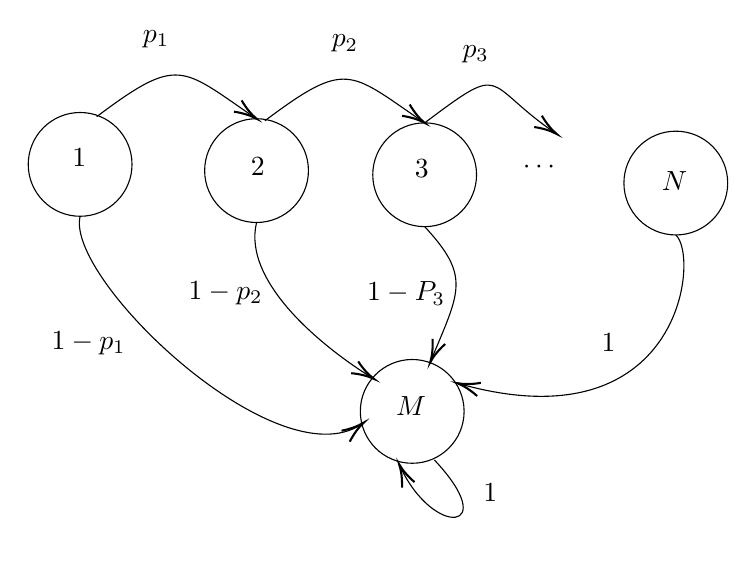
\begin{tikzpicture}[x=0.75pt,y=0.75pt,yscale=-1,xscale=1]
%uncomment if require: \path (0,300); %set diagram left start at 0, and has height of 300

%Shape: Circle [id:dp014859031609638085] 
\draw   (125,82) .. controls (125,68.19) and (136.19,57) .. (150,57) .. controls (163.81,57) and (175,68.19) .. (175,82) .. controls (175,95.81) and (163.81,107) .. (150,107) .. controls (136.19,107) and (125,95.81) .. (125,82) -- cycle ;
%Shape: Circle [id:dp10315562585513993] 
\draw   (210,85) .. controls (210,71.19) and (221.19,60) .. (235,60) .. controls (248.81,60) and (260,71.19) .. (260,85) .. controls (260,98.81) and (248.81,110) .. (235,110) .. controls (221.19,110) and (210,98.81) .. (210,85) -- cycle ;
%Shape: Circle [id:dp31422853051758903] 
\draw   (291,87) .. controls (291,73.19) and (302.19,62) .. (316,62) .. controls (329.81,62) and (341,73.19) .. (341,87) .. controls (341,100.81) and (329.81,112) .. (316,112) .. controls (302.19,112) and (291,100.81) .. (291,87) -- cycle ;
%Shape: Circle [id:dp29947365294712935] 
\draw   (412,91) .. controls (412,77.19) and (423.19,66) .. (437,66) .. controls (450.81,66) and (462,77.19) .. (462,91) .. controls (462,104.81) and (450.81,116) .. (437,116) .. controls (423.19,116) and (412,104.81) .. (412,91) -- cycle ;
%Shape: Circle [id:dp23916706575849778] 
\draw   (285,201) .. controls (285,187.19) and (296.19,176) .. (310,176) .. controls (323.81,176) and (335,187.19) .. (335,201) .. controls (335,214.81) and (323.81,226) .. (310,226) .. controls (296.19,226) and (285,214.81) .. (285,201) -- cycle ;
%Curve Lines [id:da9112509470767199] 
\draw    (158,59) .. controls (197.4,29.45) and (198.64,35.22) .. (233.39,58.91) ;
\draw [shift={(235,60)}, rotate = 214.1] [color={rgb, 255:red, 0; green, 0; blue, 0 }  ][line width=0.75]    (10.93,-3.29) .. controls (6.95,-1.4) and (3.31,-0.3) .. (0,0) .. controls (3.31,0.3) and (6.95,1.4) .. (10.93,3.29)   ;
%Curve Lines [id:da4204206989806535] 
\draw    (239,61) .. controls (278.4,31.45) and (279.64,37.22) .. (314.39,60.91) ;
\draw [shift={(316,62)}, rotate = 214.1] [color={rgb, 255:red, 0; green, 0; blue, 0 }  ][line width=0.75]    (10.93,-3.29) .. controls (6.95,-1.4) and (3.31,-0.3) .. (0,0) .. controls (3.31,0.3) and (6.95,1.4) .. (10.93,3.29)   ;
%Curve Lines [id:da6993713369170091] 
\draw    (316,62) .. controls (355.4,32.45) and (343.7,42.49) .. (378.06,66.3) ;
\draw [shift={(379.67,67.4)}, rotate = 214.1] [color={rgb, 255:red, 0; green, 0; blue, 0 }  ][line width=0.75]    (10.93,-3.29) .. controls (6.95,-1.4) and (3.31,-0.3) .. (0,0) .. controls (3.31,0.3) and (6.95,1.4) .. (10.93,3.29)   ;
%Curve Lines [id:da5910521279942383] 
\draw    (150,107) .. controls (142.74,137.1) and (244.6,234.43) .. (285.45,207.26) ;
\draw [shift={(286.67,206.4)}, rotate = 143.13] [color={rgb, 255:red, 0; green, 0; blue, 0 }  ][line width=0.75]    (10.93,-3.29) .. controls (6.95,-1.4) and (3.31,-0.3) .. (0,0) .. controls (3.31,0.3) and (6.95,1.4) .. (10.93,3.29)   ;
%Curve Lines [id:da3795671398668796] 
\draw    (235,110) .. controls (227.85,139.64) and (269.5,171.75) .. (290.12,184.46) ;
\draw [shift={(291.67,185.4)}, rotate = 210.96] [color={rgb, 255:red, 0; green, 0; blue, 0 }  ][line width=0.75]    (10.93,-3.29) .. controls (6.95,-1.4) and (3.31,-0.3) .. (0,0) .. controls (3.31,0.3) and (6.95,1.4) .. (10.93,3.29)   ;
%Curve Lines [id:da1809186903796196] 
\draw    (316,112) .. controls (338.33,136.03) and (332.84,143.19) .. (319.29,175.89) ;
\draw [shift={(318.67,177.4)}, rotate = 292.38] [color={rgb, 255:red, 0; green, 0; blue, 0 }  ][line width=0.75]    (10.93,-3.29) .. controls (6.95,-1.4) and (3.31,-0.3) .. (0,0) .. controls (3.31,0.3) and (6.95,1.4) .. (10.93,3.29)   ;
%Curve Lines [id:da29953378516051976] 
\draw    (437,116) .. controls (448.61,126.35) and (439.76,217.48) .. (333.28,187.86) ;
\draw [shift={(331.67,187.4)}, rotate = 16.02] [color={rgb, 255:red, 0; green, 0; blue, 0 }  ][line width=0.75]    (10.93,-3.29) .. controls (6.95,-1.4) and (3.31,-0.3) .. (0,0) .. controls (3.31,0.3) and (6.95,1.4) .. (10.93,3.29)   ;
%Curve Lines [id:da5272471191054172] 
\draw    (320.67,224.4) .. controls (353.17,258.87) and (320.67,262.3) .. (304.4,227.99) ;
\draw [shift={(303.67,226.4)}, rotate = 66.04] [color={rgb, 255:red, 0; green, 0; blue, 0 }  ][line width=0.75]    (10.93,-3.29) .. controls (6.95,-1.4) and (3.31,-0.3) .. (0,0) .. controls (3.31,0.3) and (6.95,1.4) .. (10.93,3.29)   ;

% Text Node
\draw (145,73.4) node [anchor=north west][inner sep=0.75pt]    {$1$};
% Text Node
\draw (231,77.4) node [anchor=north west][inner sep=0.75pt]    {$2$};
% Text Node
\draw (310,78.4) node [anchor=north west][inner sep=0.75pt]    {$3$};
% Text Node
\draw (429,84.4) node [anchor=north west][inner sep=0.75pt]    {$N$};
% Text Node
\draw (301,192.4) node [anchor=north west][inner sep=0.75pt]    {$M$};
% Text Node
\draw (362,79.4) node [anchor=north west][inner sep=0.75pt]    {$\cdots $};
% Text Node
\draw (179,16.4) node [anchor=north west][inner sep=0.75pt]    {$p_{1}$};
% Text Node
\draw (270,18.4) node [anchor=north west][inner sep=0.75pt]    {$p_{2}$};
% Text Node
\draw (333,23.4) node [anchor=north west][inner sep=0.75pt]    {$p_{3}$};
% Text Node
\draw (135,161.4) node [anchor=north west][inner sep=0.75pt]    {$1-p_{1}$};
% Text Node
\draw (201,137.4) node [anchor=north west][inner sep=0.75pt]    {$1-p_{2}$};
% Text Node
\draw (287,137.4) node [anchor=north west][inner sep=0.75pt]    {$1-P_{3}$};
% Text Node
\draw (400,162.4) node [anchor=north west][inner sep=0.75pt]    {$1$};
% Text Node
\draw (343,234.4) node [anchor=north west][inner sep=0.75pt]    {$1$};


\end{tikzpicture}

    \end{itemize}
\end{exemple}